\documentclass[tikz,border=8pt]{standalone}
\usepackage[utf8]{inputenc}
\usetikzlibrary{arrows.meta,fit,backgrounds}

% module names: smaller monospace so the longest ones fit in a block
\newcommand{\modname}[1]{{\scriptsize\ttfamily #1}}

\begin{document}
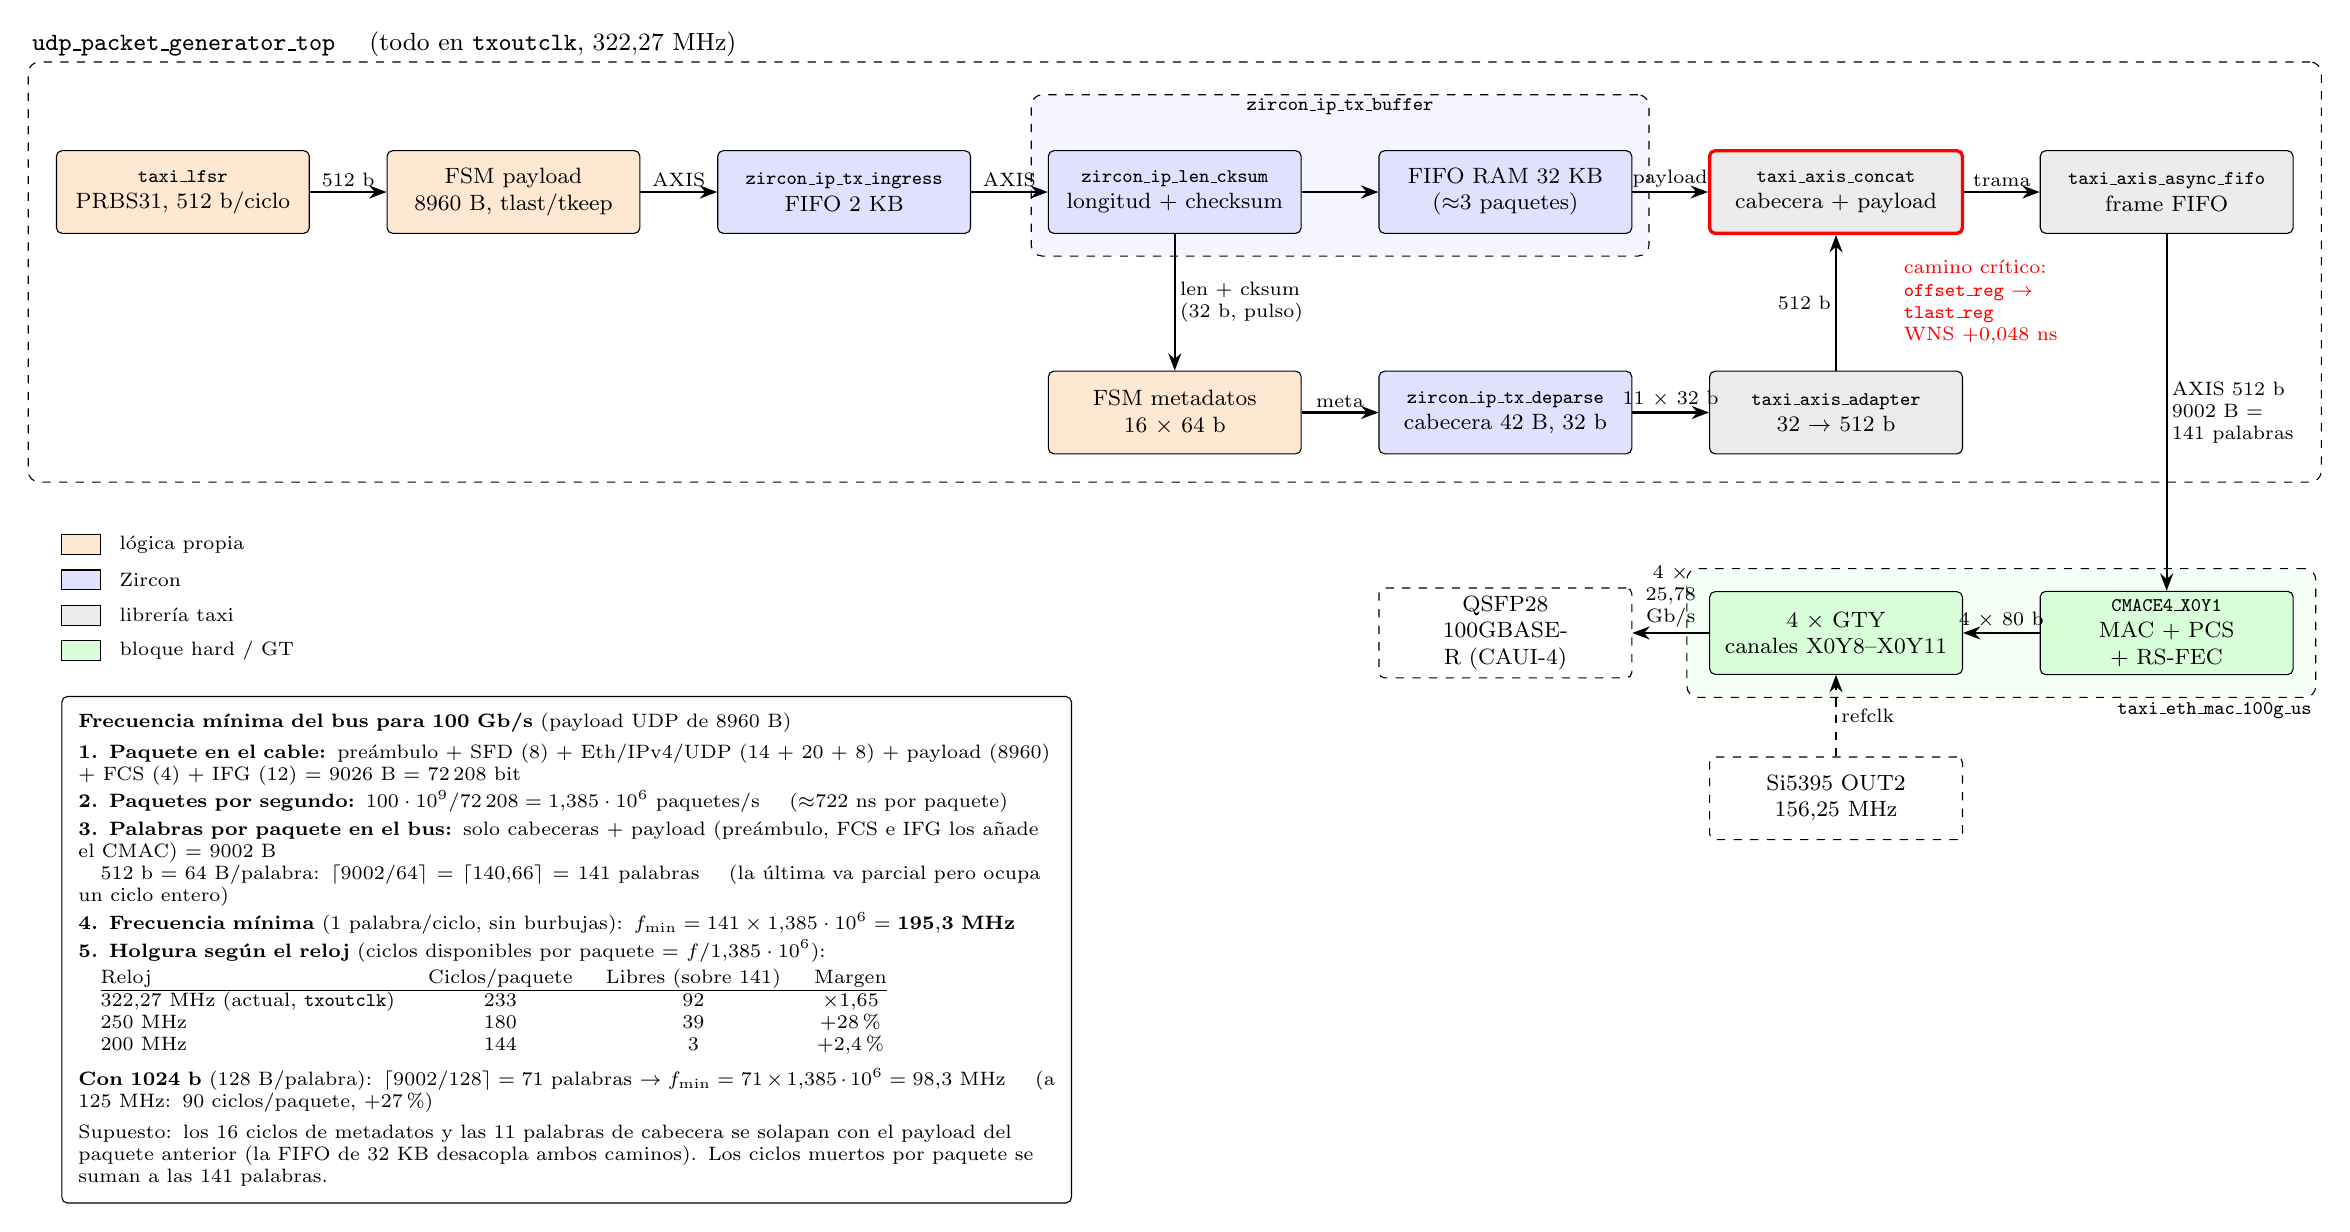
\begin{tikzpicture}[
    x=1.235cm,
    font=\footnotesize,
    >={Stealth[length=2.2mm]},
    blk/.style={draw, rounded corners=2pt, minimum height=1.05cm,
                text width=3.0cm, align=center, inner sep=3pt},
    gen/.style={blk, fill=orange!18},
    zir/.style={blk, fill=blue!12},
    taxi/.style={blk, fill=gray!15},
    hard/.style={blk, fill=green!15},
    ext/.style={blk, fill=white, dashed},
    grp/.style={draw, dashed, rounded corners=4pt},
    lbl/.style={font=\scriptsize, inner sep=1.5pt},
    flow/.style={->, thick},
]

% ---------------------------------------------------------------- payload path
\node[gen]  (lfsr)    at (0,0)     {\modname{taxi\_lfsr}\\PRBS31, 512 b/ciclo};
\node[gen]  (fsmp)    at (3.4,0)   {FSM payload\\8960 B, tlast/tkeep};
\node[zir]  (ingress) at (6.8,0)   {\modname{zircon\_ip\_tx\_ingress}\\FIFO 2 KB};
\node[zir]  (cksum)   at (10.2,0)  {\modname{zircon\_ip\_len\_cksum}\\longitud + checksum};
\node[zir]  (ram)     at (13.6,0)  {FIFO RAM 32 KB\\($\approx$3 paquetes)};
\node[taxi, draw=red, very thick]
            (concat)  at (17,0)    {\modname{taxi\_axis\_concat}\\cabecera + payload};
\node[taxi] (afifo)   at (20.4,0)  {\modname{taxi\_axis\_async\_fifo}\\frame FIFO};

% ---------------------------------------------------------------- metadata path
\node[gen]  (fsmm)    at (10.2,-2.8) {FSM metadatos\\16 $\times$ 64 b};
\node[zir]  (deparse) at (13.6,-2.8) {\modname{zircon\_ip\_tx\_deparse}\\cabecera 42 B, 32 b};
\node[taxi] (adapter) at (17,-2.8)   {\modname{taxi\_axis\_adapter}\\32 $\to$ 512 b};

% ---------------------------------------------------------------- MAC / PHY
\node[hard] (cmac)    at (20.4,-5.6) {\modname{CMACE4\_X0Y1}\\MAC + PCS + RS-FEC};
\node[hard] (gty)     at (17,-5.6)   {4 $\times$ GTY\\canales X0Y8--X0Y11};
\node[ext]  (qsfp)    at (13.6,-5.6) {QSFP28\\100GBASE-R (CAUI-4)};
\node[ext]  (si5395)  at (17,-7.7)   {Si5395 OUT2\\156,25 MHz};

% ---------------------------------------------------------------- arrows
\draw[flow] (lfsr)    -- node[lbl, above] {512 b} (fsmp);
\draw[flow] (fsmp)    -- node[lbl, above] {AXIS} (ingress);
\draw[flow] (ingress) -- node[lbl, above] {AXIS} (cksum);
\draw[flow] (cksum)   -- (ram);
\draw[flow] (ram)     -- node[lbl, above] {payload} (concat);
\draw[flow] (concat)  -- node[lbl, above] {trama} (afifo);

\draw[flow] (cksum)   -- node[lbl, right, text width=1.9cm] {len + cksum\\(32 b, pulso)} (fsmm);
\draw[flow] (fsmm)    -- node[lbl, above] {meta} (deparse);
\draw[flow] (deparse) -- node[lbl, above] {11 $\times$ 32 b} (adapter);
\draw[flow] (adapter) -- node[lbl, left] {512 b} (concat);

\draw[flow] (afifo)   -- node[lbl, right, text width=1.6cm] {AXIS 512 b\\9002 B =\\141 palabras} (cmac);
\draw[flow] (cmac)    -- node[lbl, above] {4 $\times$ 80 b} (gty);
\draw[flow] (gty)     -- node[lbl, above, text width=1cm, align=center] {4 $\times$ 25,78\\Gb/s} (qsfp);
\draw[flow, dashed] (si5395) -- node[lbl, right] {refclk} (gty);

% critical path
\node[lbl, text=red, text width=2.6cm, align=left] at (18.75,-1.4)
    {camino crítico:\\\texttt{offset\_reg} $\to$\\\texttt{tlast\_reg}\\WNS +0,048 ns};

% ---------------------------------------------------------------- groups
\coordinate (gentop) at (0,1.3);
\begin{scope}[on background layer]
    \node[grp, fit=(cksum)(ram), inner xsep=6pt, inner ysep=14pt, yshift=6pt,
          fill=blue!4] (bufgrp) {};
    \node[grp, fit=(gentop)(lfsr)(afifo)(adapter), inner sep=10pt] (gengrp) {};
    \node[grp, fit=(gty)(cmac), inner sep=8pt, fill=green!4] (macgrp) {};
\end{scope}
\node[lbl, anchor=north] at (bufgrp.north) {\texttt{zircon\_ip\_tx\_buffer}};
\node[lbl, anchor=south west, font=\small] at (gengrp.north west)
    {\texttt{udp\_packet\_generator\_top} \quad (todo en \texttt{txoutclk}, 322,27 MHz)};
\node[lbl, anchor=north east] at (macgrp.south east) {\texttt{taxi\_eth\_mac\_100g\_us}};

% ---------------------------------------------------------------- legend
\begin{scope}[shift={(-1.25,-4.6)}, every node/.style={font=\scriptsize, anchor=west}]
    \draw[fill=orange!18] (0,0)     rectangle +(0.4,0.25); \node at (0.5,0.125)  {lógica propia};
    \draw[fill=blue!12]   (0,-0.45) rectangle +(0.4,0.25); \node at (0.5,-0.325) {Zircon};
    \draw[fill=gray!15]   (0,-0.9)  rectangle +(0.4,0.25); \node at (0.5,-0.775) {librería taxi};
    \draw[fill=green!15]  (0,-1.35) rectangle +(0.4,0.25); \node at (0.5,-1.225) {bloque hard / GT};
\end{scope}

\node[draw, rounded corners=2pt, anchor=north west, text width=12.4cm, align=left,
      font=\scriptsize, inner sep=6pt] at (-1.25,-6.4) {%
    \textbf{Frecuencia mínima del bus para 100 Gb/s} (payload UDP de 8960 B)\\[3pt]
    \textbf{1. Paquete en el cable:}
    preámbulo + SFD (8) + Eth/IPv4/UDP (14 + 20 + 8) + payload (8960) + FCS (4) + IFG (12)
    = 9026 B = 72\,208 bit\\[2pt]
    \textbf{2. Paquetes por segundo:}
    $100\cdot10^{9} / 72\,208 = 1{,}385\cdot10^{6}$ paquetes/s
    \quad($\approx$722 ns por paquete)\\[2pt]
    \textbf{3. Palabras por paquete en el bus:}
    solo cabeceras + payload (preámbulo, FCS e IFG los añade el CMAC) = 9002 B\\
    \hspace*{1em}512 b = 64 B/palabra: $\lceil 9002/64 \rceil = \lceil 140{,}66 \rceil = 141$ palabras
    \quad(la última va parcial pero ocupa un ciclo entero)\\[2pt]
    \textbf{4. Frecuencia mínima} (1 palabra/ciclo, sin burbujas):
    $f_{\min} = 141 \times 1{,}385\cdot10^{6} = \mathbf{195{,}3\ MHz}$\\[2pt]
    \textbf{5. Holgura según el reloj} (ciclos disponibles por paquete = $f / 1{,}385\cdot10^{6}$):\\[1pt]
    \hspace*{1em}\begin{tabular}{@{}lccc@{}}
        Reloj & Ciclos/paquete & Libres (sobre 141) & Margen\\\hline
        322,27 MHz (actual, \texttt{txoutclk}) & 233 & 92 & $\times$1,65\\
        250 MHz & 180 & 39 & +28\,\%\\
        200 MHz & 144 & 3 & +2,4\,\%\\
    \end{tabular}\\[3pt]
    \textbf{Con 1024 b} (128 B/palabra): $\lceil 9002/128 \rceil = 71$ palabras
    $\to f_{\min} = 71 \times 1{,}385\cdot10^{6} = 98{,}3$ MHz
    \quad(a 125 MHz: 90 ciclos/paquete, +27\,\%)\\[3pt]
    Supuesto: los 16 ciclos de metadatos y las 11 palabras de cabecera se solapan con el payload
    del paquete anterior (la FIFO de 32 KB desacopla ambos caminos). Los ciclos muertos
    por paquete se suman a las 141 palabras.};

\end{tikzpicture}
\end{document}
